%%%%%%%%%%%%%%%%%%%%%%%%%%%%%%%%%%%%%%%%%%%%%%%%%%%%%%%%
%%%%%%                                            %%%%%%
%%%                                                  %%%
%      Modèle de Rapport.                              %
%               Par Matthieu Maury                     %
%                                                      %
%%%                                                  %%%
%%%%%%                                            %%%%%%
%%%%%%%%%%%%%%%%%%%%%%%%%%%%%%%%%%%%%%%%%%%%%%%%%%%%%%%%

\documentclass[10pt, a4paper]{report}

%%%%%%%%%%%%%%%%%%%%%%%%%%%%%%%%%%%%%%%%%%%%%%%%%%%%%%%%
%% Package essentiel
\usepackage[greek,english]{babel}
\usepackage[T1]{fontenc}
\usepackage{ucs}
\usepackage[utf8x]{inputenc}
\usepackage[top=2.6cm,bottom=2.6cm,right=2.1cm,left=2.1cm]{geometry}
\usepackage{float}

%%%%%%%%%%%%%%%%%%%%%%%%%%%%%%%%%%%%%%%%%%%%%%%%%%%%%%%%
%% Package optionnel
\usepackage{enumerate}
\usepackage{graphicx}
\usepackage{tabularx}
\usepackage{setspace}
\usepackage[dvips]{pstricks}
\usepackage{pstricks-add}
\usepackage{color}
\usepackage{xcolor}
\usepackage{epsfig}
\usepackage{pst-grad} % For gradients
\usepackage{pst-plot} % For axes
\usepackage{amsmath}
\usepackage{amsfonts}
\usepackage{amssymb}
\usepackage{amsxtra}
\usepackage{mathrsfs}
\usepackage{framed}
%\usepackage[framed, thmmarks, amsmath]{ntheorem}
\usepackage{verbatim}
\usepackage{moreverb}
\usepackage{fancyhdr}
\usepackage{url}
\usepackage{listings}
%\usepackage{hyperlinks}
\usepackage{lettrine}

%%%%%%%%%%%%%%%%%%%%%%%%%%%%%%%%%%%%%%%%%%%%%%%%%%%%%%%%
%%%%%%                                            %%%%%%
%%         Configuration de la mise en page           %%
%%%%%                                              %%%%%
%%%%%%%%%%%%%%%%%%%%%%%%%%%%%%%%%%%%%%%%%%%%%%%%%%%%%%%%

%%%%%%%%%%%%%%%%%%%%%%%%%%%%%%%%%%%%%%%%%%%%%%%%%%%%%%%%
%% Profondeur du sommaire
\setcounter{secnumdepth}{4}
\setcounter{tocdepth}{4}

%%%%%%%%%%%%%%%%%%%%%%%%%%%%%%%%%%%%%%%%%%%%%%%%%%%%%%%%
%% Configuration des chapitres
\makeatletter
\def\@makechapterhead#1{%
  \vspace*{50\p@}%
  {\parindent \z@ \raggedright \normalfont
    \interlinepenalty\@M
    \Huge \bfseries\thechapter.\quad#1\par\nobreak
    \vskip 20\p@
  }}
\makeatother

%%%%%%%%%%%%%%%%%%%%%%%%%%%%%%%%%%%%%%%%%%%%%%%%%%%%%%%%
%%%%%%                                            %%%%%%
%%                Début du Document                   %%
%%%%%                                              %%%%%
%%%%%%%%%%%%%%%%%%%%%%%%%%%%%%%%%%%%%%%%%%%%%%%%%%%%%%%%


\lstset{tabsize=3, inputencoding=utf8x, extendedchars=\true, language=C}

%% Symboles des ensembles
\newcommand{\R}{\ensuremath{\mathbb{R}} }
\newcommand{\N}{\ensuremath{\mathbb{N}} }
\newcommand{\Z}{\ensuremath{\mathbb{Z}} }
\newcommand{\Q}{\ensuremath{\mathbb{Q}} }
\newcommand{\C}{\ensuremath{\mathbb{C}} }
\newcommand{\U}{\ensuremath{\mathbb{U}} }
\newcommand{\K}{\ensuremath{\mathbb{K}} }

%% Symboles mathématique
\newcommand{\spi}{\ensuremath{\Pi} } %Pi
\newcommand{\sqqs}{\ensuremath{\forall} } %quelque sois
\newcommand{\sex}{\ensuremath{\exists} } %il existe
\newcommand{\snex}{\ensuremath{\nexists} }
\newcommand{\simpld}{\ensuremath{\Rightarrow} } %implique vers la droite
\newcommand{\simplg}{\ensuremath{\Leftarrow} } %implque vers la gauche
\newcommand{\sequ}{\ensuremath{\Leftrightarrow} }
\newcommand{\sand}{\ensuremath{\wedge} }
\newcommand{\sou}{\ensuremath{\vee} }
\newcommand{\smneg}{\ensuremath{\neg} }
\newcommand{\snimpld}{\ensuremath{\nRightarrow} } %implique vers la droite
\newcommand{\snimplg}{\ensuremath{\nLeftarrow} } %implque vers la gauche
\newcommand{\snequ}{\ensuremath{\nLeftrightarrow} }
\newcommand{\sinclut}{\ensuremath{\in} }
\newcommand{\sninclut}{\ensuremath{\notin} }
\newcommand{\sposd}{\ensuremath{\owns} }
\newcommand{\ssups}{\ensuremath{\supset} }
\newcommand{\snsups}{\ensuremath{\nsupset} }
\newcommand{\ssubs}{\ensuremath{\subset} }
\newcommand{\ssubeq}{\ensuremath{\subseteq} }
\newcommand{\ssupeq}{\ensuremath{\supseteq} }
\newcommand{\snsubeq}{\ensuremath{\nsubseteq} }
\newcommand{\snsupeq}{\ensuremath{\nsupseteq} }
\newcommand{\sneg}{\ensuremath{\neq} }
\newcommand{\saprox}{\ensuremath{\approx} }
\newcommand{\ssim}{\ensuremath{\sim} }
\newcommand{\scompl}[2]{\ensuremath{\complement_{#1}{#2}} }
\newcommand{\sunion}{\ensuremath{\cup} }
\newcommand{\sinters}{\ensuremath{\cap} }
\newcommand{\sx}{\ensuremath{\times} }
\newcommand{\svide}{\ensuremath{\emptyset} }
\newcommand{\Pa}{\ensuremath{\mathcal{P}} }
\newcommand{\lra}{\ensuremath{\longrightarrow}}
\newcommand{\rond}{\ensuremath{\circ} }
\newcommand{\frestric}[2]{\ensuremath{#1|_{#2}} }
\newcommand{\sbar}[1]{\ensuremath{\overline{#1}}}
\newcommand{\si}{\ensuremath{\imath}}
\newcommand{\zl}[1]{\ensuremath{\mathscr{#1}}}
\newcommand{\stimes}{\ensuremath{\times}}
\newcommand{\classe}[1]{\ensuremath{\overset{\bullet}{#1}}}


\begin{document}

%%%%%%%%%%%%%%%%%%%%%%%%%%%%%%%%%%%%%%%%%%%%%%%%%%%%%%%%
%% Inclusion de la page de titre
\pagestyle{fancy}
\renewcommand{\sectionmark}[1]{\markright{\thesection\ #1}}
\renewcommand{\footrulewidth}{0pt}
\renewcommand{\headrulewidth}{0pt}
\fancyhead{} % clear all header fields
\fancyfoot{} % clear all footer fields
\fancyfoot[LO,RE]{\textit{University year 2009-2010}}
\fancyfoot[LE,RO]{\textit{Written with \LaTeX}}

\begin{tabularx}{17cm}{Xr}
  \begin{tabular}{ll}
	 Matthieu Maury & 860928-P210\\
	 \url{mayeu.tik@gmail.com} & \\
	 Yohann Teston & 881003-P792\\
	 \url{yohann.teston@free.fr} &\\
  \end{tabular} 

  &

  \begin{tabular}{r}
	 
\includegraphics[width=5cm]{pic/logoupp.eps} \\
	 \textit{Department of Information Technology} \\
  \end{tabular}
\end{tabularx}

\vspace{6cm}

\begin{center}
  \textbf{ {\Huge Programming of parallel computers}}\\[0.5em]{\huge Lab 3 - OpenMP}
\end{center}

\begin{center}
  \today
\end{center}

\newpage


\thispagestyle{empty}
%\input{resume}

\renewcommand{\footrulewidth}{0.5pt}
\renewcommand{\headrulewidth}{0.5pt}
\fancyhead{} % clear all header fields
\fancyhead[RE,LO]{Programming of parallel computers - Lab 3 - OpenMP}


\fancyhead[RO,LE]{\rightmark}

\fancyfoot{} % clear all footer fields
\fancyfoot[LO,RE]{Matthieu Maury \& Yohann Teston}
\fancyfoot[LE,RO]{\thepage}

%Redéfinition du style fancy - plain, utilisé pour les pages de nouveau chapitre
%Le style par défaut est un style plain
\fancypagestyle{plain}{
    \fancyhf{}
    \renewcommand{\headrulewidth}{0pt}

    %Définition des headers identiques à une page normale
    \fancyfoot[LO,RE]{Matthieu Maury \& Yohann Teston}
    \fancyfoot[LE,RO]{\thepage}
}

\tableofcontents

%\listoffigures

%\newpage

%\doublespacing
\onehalfspacing
\chapter{Compile and run OpenMP programs}

\begin{verbatim}
$ export OMP_NUM_THREADS=4 ; ./helloworld
Starting
4 threads involved
Thread 0: Hello World!
Thread 3: Hello World!
Thread 1: Hello World!
Thread 2: Hello World!
Stopping
\end{verbatim}

As we can expect the thread don't have any specific order. Again this is due to the thread scheduller


\chapter{Data sharing}

We can assume that $a$ will be equal to 10 after the datasharing program:
\begin{verbatim}
$ ./datasharing 
a= 10 b= 10
a= 10 b= 10
a= 10 b= 10
a= 10 b= 10
\end{verbatim}

As we see every thread modifies its own $a$ locally, so they do not use the first initialization of $a$. Therefore, the $a$ manipulated by the threads is not the global $a$ but a local variable (which was not initialized). 
After adding the $firstprivate$ pragma, we can expect that $a$ will be added $10$ once in each thread, but this time starting from $a = 10$, because the local $a$ is initialized with the value of the global $a$:

\begin{verbatim}
$ ./datasharing 
a= 20 b= 10
a= 20 b= 10
a= 20 b= 10
a= 20 b= 10
\end{verbatim}

We see that $a$ is now initialized to 10 and equals to $20$ at the end because the calculus $a += b$ is made in every thread.

\chapter{Work sharing}

\section{Unmodified program}

\begin{figure}[!h]
  \begin{center}
         \resizebox{160mm}{!}{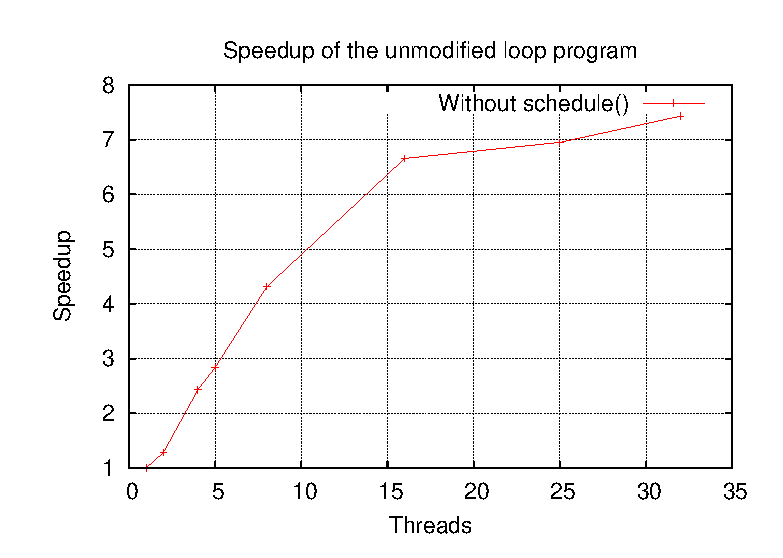
\includegraphics{pic/graph_q4.eps}}
  \end{center}
  \caption{Speedup of the unmodified program}
  \label{unmodif}
\end{figure}

The speedup keeps increasing slowly but is too low for a few threads to jusitfy their use.

\section{Using scheduling directives}

In the graphs \ref{2000} and \ref{10000}, we tried the three directives with an arbitrary sized chunk. The graph \ref{opt} shows the result if we let OpenMP take care of the chunk's size.

\begin{figure}[!h]
  \begin{center}
         \resizebox{160mm}{!}{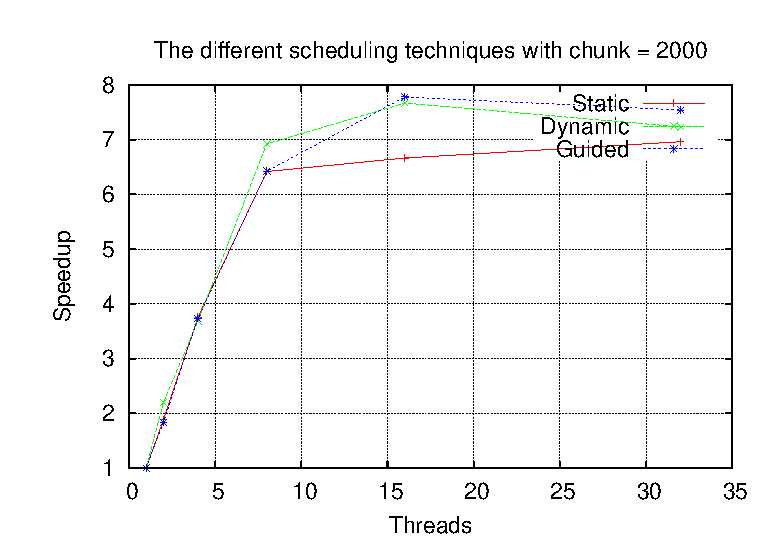
\includegraphics{pic/graph_q4_2000.eps}}
  \end{center}
  \caption{With chunk = 2000}
  \label{2000}
\end{figure}

\begin{figure}[!h]
  \begin{center}
         \resizebox{160mm}{!}{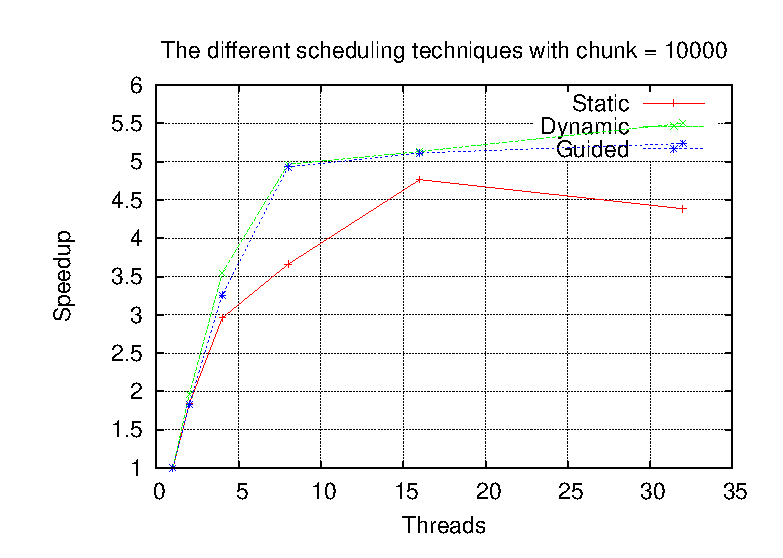
\includegraphics{pic/graph_q4_10000.eps}}
  \end{center}
  \caption{With chunk = 10000}
  \label{10000}
\end{figure}

\begin{figure}[!h]
  \begin{center}
         \resizebox{160mm}{!}{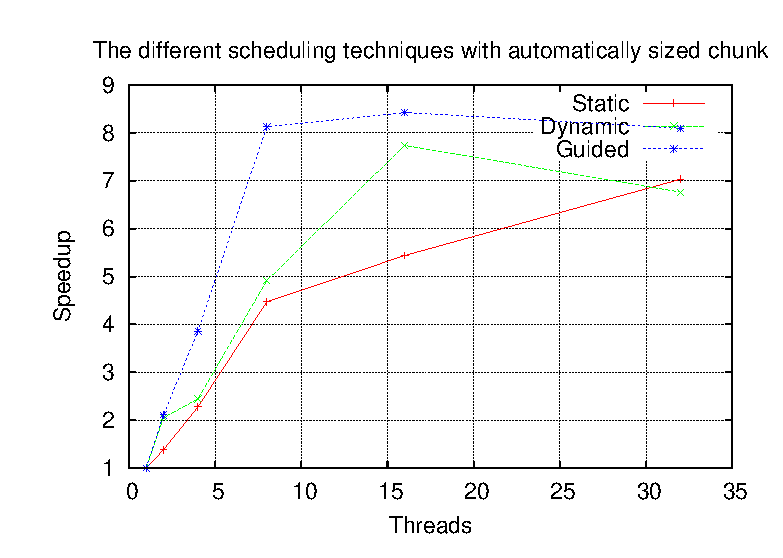
\includegraphics{pic/graph_q4_opt.eps}}
  \end{center}
  \caption{With automatically sized chunk}
  \label{opt}
\end{figure}


The chunk size is important. If is is too big, it will create load imbalance and lead to bad results, as the picture \ref{10000} shows. Too small chunks are not good either as they multiply the number of context switches. 

As we can see, especially with automatically sized chunks,  choosing dynamic or guided scheduling gives the bests results. It is so because the problem was a poor load balance and it is known that both dynamic and guided scheduling are good to avoid this problem. Both dynamic and guided scheduling have very good results with a few number of threads, very close to the optimal speedup (which is simply the number of processors involved). This is not the case of the static scheduling. However, the results start to stagnate passed the 10 threads involved. This is caused by the fact that our problem size does not scale but the overhead keeps increasing.


\chapter{Examples}

\section{$\pi$}

The code for this program is available in the appendix \ref{pi}.

\section{Enumeration sort}

The plot \ref{enumsort_plot} presents the speedup got parallelizing the differents loops.

\begin{figure}[!h]
  \begin{center}
%         \resizebox{160mm}{!}{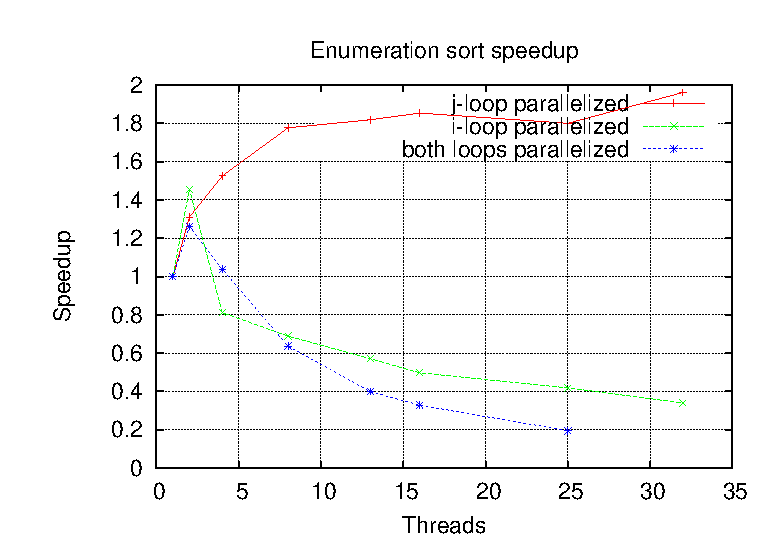
\includegraphics{pic/graph_enumsort.eps}}
  \end{center}
  \caption{enumeration sort's speedup}
  \label{enumsort_plot}
\end{figure} 

As we can see, the results are really bad when either the i-loop or both lopps are parallelized. In this case, the more threads we have, the more time we need to complete. We can also underline the fact that the program takes more time in that case than that it takes with only one thread.

The only "good" result is given by parallelizing the j-loop only. Even in this case, the result are quite bad with a speedup less than 2 using 32 threads.

This can be explained by the fact that the threads synchronize among them a lot, especially in the two last cases.

When only the j-loop is parallelized, there is only one barrier at the end of the loop, that is one barrier in the whole program. So, the threads have to synchronize, and that hinders the performances, but only once. Thus, it is still possible to achieve better performances.

However, in the case where the i-loop is parallelized, there is a barrier at the end of this loop. The problem comes from the fact that this loop is nested in the j-loop. So, there is a barrier for each iteration. Besides, there is a reduction operation. Thus, there is also some communication going on at that step. The time lost synchronizing the threads for each iteration and passing data around explains the bad results.

The very bad results at the last experiment are explained in the same way as above but this time both of the mentioned inconveniences are present. Because of the nested parallelization, the outer loop is divided among the threads but so is the inner loop. Therefore, there is again a lot of time wasted waiting for the others, hence the results.     

\newpage
\setcounter{page}{1}
\pagenumbering{Roman}
\appendix
\chapter{Compile and run OpenMP programs}

\lstinputlisting{../labOpenMP/helloworld.c}

\chapter{Data Sharing}

\lstinputlisting{../labOpenMP/datasharing.c}

\chapter{Reduce}
\lstinputlisting{../labOpenMP/reduce.c}
\label{reduce}

\chapter{Example}

\section{$\pi$}
\lstinputlisting{../labOpenMP/pi.c}
\label{pi}

\section{Enumeration sort}
\lstinputlisting{../labOpenMP/enumsort_2.c}
\label{enumsort}

\chapter{LU-factorization, an advanced example}

\lstset{tabsize=3, inputencoding=utf8x, extendedchars=\true, language=Fortran}

\section{lu.f90}
\lstinputlisting{../labOpenMP/lu.f90}

\section{lulock.f90}
\lstinputlisting{../labOpenMP/lulock.f90}


\end{document}
